\documentclass[12pt,letterpaper]{article}
\usepackage{graphicx,textcomp}
\usepackage{natbib}
\usepackage{setspace}
\usepackage{fullpage}
\usepackage{color}
\usepackage[reqno]{amsmath}
\usepackage{amsthm}
\usepackage{fancyvrb}
\usepackage{amssymb,enumerate}
\usepackage[all]{xy}
\usepackage{endnotes}
\usepackage{lscape}
\newtheorem{com}{Comment}
\usepackage{float}
\usepackage{hyperref}
\newtheorem{lem} {Lemma}
\newtheorem{prop}{Proposition}
\newtheorem{thm}{Theorem}
\newtheorem{defn}{Definition}
\newtheorem{cor}{Corollary}
\newtheorem{obs}{Observation}
\usepackage[compact]{titlesec}
\usepackage{dcolumn}
\usepackage{tikz}
\usetikzlibrary{arrows}
\usepackage{multirow}
\usepackage{xcolor}
\newcolumntype{.}{D{.}{.}{-1}}
\newcolumntype{d}[1]{D{.}{.}{#1}}
\definecolor{light-gray}{gray}{0.65}
\usepackage{url}
\usepackage{listings}
\usepackage{color}

\definecolor{codegreen}{rgb}{0,0.6,0}
\definecolor{codegray}{rgb}{0.5,0.5,0.5}
\definecolor{codepurple}{rgb}{0.58,0,0.82}
\definecolor{backcolour}{rgb}{0.95,0.95,0.92}

\lstdefinestyle{mystyle}{
	backgroundcolor=\color{backcolour},   
	commentstyle=\color{codegreen},
	keywordstyle=\color{magenta},
	numberstyle=\tiny\color{codegray},
	stringstyle=\color{codepurple},
	basicstyle=\footnotesize,
	breakatwhitespace=false,         
	breaklines=true,                 
	captionpos=b,                    
	keepspaces=true,                 
	numbers=left,                    
	numbersep=5pt,                  
	showspaces=false,                
	showstringspaces=false,
	showtabs=false,                  
	tabsize=2
}
\lstset{style=mystyle}
\newcommand{\Sref}[1]{Section~\ref{#1}}
\newtheorem{hyp}{Hypothesis}

\title{Problem Set 4}
\date{Due: April 16, 2023}
\author{Applied Stats II}


\begin{document}
	\maketitle
	\section*{Instructions}
	\begin{itemize}
	\item Please show your work! You may lose points by simply writing in the answer. If the problem requires you to execute commands in \texttt{R}, please include the code you used to get your answers. Please also include the \texttt{.R} file that contains your code. If you are not sure if work needs to be shown for a particular problem, please ask.
	\item Your homework should be submitted electronically on GitHub in \texttt{.pdf} form.
	\item This problem set is due before 23:59 on Sunday April 16, 2023. No late assignments will be accepted.

	\end{itemize}

	\vspace{.25cm}
\section*{Question 1}
\vspace{.25cm}
\noindent \textit{We're interested in modeling the historical causes of child mortality. We have data from 26855 children born in Skellefteå, Sweden from 1850 to 1884. Using the "child" dataset in the \texttt{eha} library, fit a Cox Proportional Hazard model using mother's age and infant's gender as covariates. Present and interpret the output.} \\

\noindent First, the data was imported, after which a Cox Proportional Hazard Regression model was fit to the data:

\lstinputlisting[language=R, firstline=15, lastline=19]{code/coxreg.R} 

\noindent This gave the following output:

\begin{table}[!htbp] \centering 
	\caption{Cox Proportional Hazard Regression} 
	\label{} 
	\begin{tabular}{@{\extracolsep{5pt}}lc} 
		\\[-1.8ex]\hline 
		\hline \\[-1.8ex] 
		& \multicolumn{1}{c}{\textit{Dependent variable:}} \\ 
		\cline{2-2} 
		\\[-1.8ex] & enter \\ 
		\hline \\[-1.8ex] 
		sexfemale & $-$0.082$^{***}$ \\ 
		& (0.027) \\ 
		& \\ 
		m.age & 0.008$^{***}$ \\ 
		& (0.002) \\ 
		& \\ 
		\hline \\[-1.8ex] 
		Observations & 26,574 \\ 
		R$^{2}$ & 0.001 \\ 
		Max. Possible R$^{2}$ & 0.986 \\ 
		Log Likelihood & $-$56,503.480 \\ 
		Wald Test & 22.520$^{***}$ (df = 2) \\ 
		LR Test & 22.518$^{***}$ (df = 2) \\ 
		Score (Logrank) Test & 22.530$^{***}$ (df = 2) \\ 
		\hline 
		\hline \\[-1.8ex] 
		\textit{Note:}  & \multicolumn{1}{r}{$^{*}$p$<$0.1; $^{**}$p$<$0.05; $^{***}$p$<$0.01} \\ 
	\end{tabular} 
\end{table} 

\vspace{5in}
\noindent As can be seen, both of the covariates had significant effects on the log of the hazard, being the death of the child. In the case of the sex covariate, holding the age of the mother constant, there is a .08 decrease in the expected log of the hazard when the baby is female. This means that the hazard ratio for female babies is 0.92 to that of the male babies, meaning female deaths are lower by 8\% compared to that of male babies \\

\noindent Holding sex constant, for every year increase in the mother's age, there is a .008 increase in the log of the hazard being the death of the child. This means that for every year increase in the mother's age, there is a 0.7\% increase in the expected hazard, being the death of their child. \\

\noindent A likelihood ratio test was also carried out to assess whether the model is more useful than a null model. As shown in Table 2, the results indicate that using both covariates are more useful than a null model, with the p values being less than 0.05 for both. \\

\begin{table}[!htbp] \centering 
	\caption{Likelihood Ratio Test} 
	\label{} 
	\begin{tabular}{@{\extracolsep{5pt}} ccccc} 
		\\[-1.8ex]\hline 
		\hline \\[-1.8ex] 
		& Df & AIC & LRT & Pr(\textgreater Chi) \\ 
		\hline \\[-1.8ex] 
		\textless none\textgreater  & $$ & $113,011.000$ & $$ & $$ \\ 
		sex & $1$ & $113,018.400$ & $9.465$ & $0.002$ \\ 
		m.age & $1$ & $113,021.800$ & $12.795$ & $0.0003$ \\ 
		\hline \\[-1.8ex] 
	\end{tabular} 
\end{table} 

\noindent Using this model, we can plot the Cumulative Hazard Function, indicating the probability of the hazard occurring as the time passed, as shown in Figure 1.

\begin{figure}
	\centering
	
	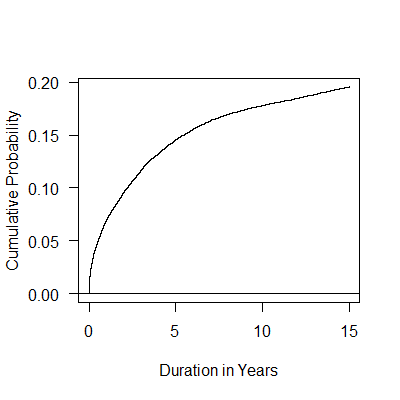
\includegraphics[width=6in]{chf.png}
	\caption{Cumulative Hazard Function - Cumulative Probability of Death Occurring as Child Ages}
	
\end{figure}
\end{document}
